%!TEX root = ./template-skripsi.tex
%-------------------------------------------------------------------------------
%                            BAB III
%               			PEMBAHASAN
%-------------------------------------------------------------------------------

\chapter{IMPLEMENTASI PROGRAM}


\section{Tahapan Penelitian}

\begin{figure}[H]
	\centering
	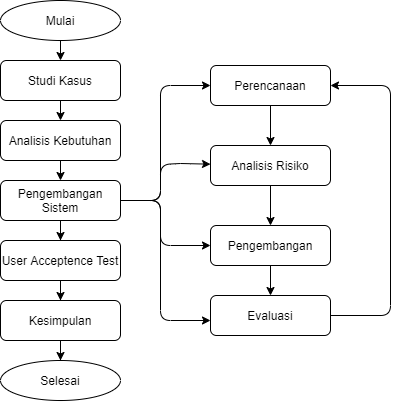
\includegraphics[width=0.8\textwidth]{gambar/diagram/flowchart}
	\caption{\textit{Flowchart} tahapan penelitian}
	\label{fig:flow}
\end{figure}

Tahapan penelitian terdiri dari beberapa proses yang dimulai dari studi kasus yang merupakan sebuah proses dimana penulis melakukan studi permasalahan umum yang ada pada monitoring kegiatan belajar mengajar. Analisis Kebutuhan adalah tahapan dimana penulis menganalisis kebutuhan dari sistem yang akan dibuat dengan cara wawancara. Pengembangan sistem adalah tahapan pengembangan sistem itu sendiri yang penulis lakukan dengan menerapkan metodologi Spiral. \textit{User Acceptance Test} adalah tahapan \textit{testing} yang dilakukan untuk mengetahui apakai sistem yang telah dibuat sesuai dengan kebutuhan dan tujuan pembuatannya. Tahapan terakhir adalah penarikan kesimpulan.

\section{Analisis Kebutuhan}
Pada tahapan ini, penulis mengumpulkan informasi tentang kebutuhan dari perangkat lunak yang akan dikembangkan dengan cara mewawancara beberapa pihak seperti Koordinator Program Studi, Tim Penjamin Mutu Prodi, dan Gugus Penjamin Mutu FMIPA yang dapat dilihat pada Lampiran A. Penulis juga mengumpulkan informasi dari pengumpulan data pada penelitian serupa yang sebelumnya pernah dilakukan yaitu penelitian yang dilakukan oleh \cite{FitriAndiniMedIrzal2017} yang berjudul "Perancangan dan Implementasi Sistem Absensi Online Berbasis Android di Linkungan Universitas Negeri Jakarta"  dan \cite{Kultsum2021} yang berjudul ''Rancang Bangun Sistem Presensi Akademik Berbasis Web Dengan \textit{Framework} Laravel di Lingkungan Program Studi Ilmu Komputer Universitas Negeri Jakarta''. Berikut beberapa hasil kebutuhan yang penulis dapatkan:

\begin{enumerate}
	\item Sistem memiliki lima jenis pengguna yaitu mahasiswa, penanggung jawab mata kuliah, dosen, tim penjamin mutu, dan admin.
	\item Mahasiswa dapat melihat kelas-kelas yang diambil, mengisi presensi ketika sudah ada pertemuan atau form 05 yang diisi oleh penanggung jawab atau dosen, dan melihat nilai tugas-tugas yang telah diisi oleh dosen.
	\item Penanggung jawab mata kuliah adalah bagian dari mahasiswa dengan tugas tambahan yaitu  mengisi atau memvalidasi form 05. Penanggung jawab mata kuliah dipilih oleh dosen pada pertemuan pertama.
	\item Dosen dapat melihat kelas-kelas yang diampu, mengisi form 05 untuk pertemuan pada kelas tersebut, dan dapat menutup waktu presensi untuk mahasiswa. Untuk memvalidasi presensi dari mahasiswa Dosen dapat memilih untuk memvalidasi semua presensi yang masuk, melakukan seleksi validasi presensi yang sudah masuk, atau memvalidasi semua presensi yang masuk sebelum waktu yang ditentukan.  Dosen juga dapat menambahkan tugas dan mengisi nilai tugas setiap mahasiswa dengan mengunduh format excel yang telah tersedia dan mengunggah \textit{file excel} tersebut ketika ada pembaruan. Ketika penanggung jawab mata kuliah tidak bisa hadir, dosen juga dapat menunjuk penanggung jawab mata kuliah sementara untuk pertemuan tersebut.
	\item Tim penjamin mutu adalah bagian dari dosen dengan tambahan yaitu memiliki menu monitoring yang berisi informasi semua kelas-kelas pada program studi termasuk yang tidak diampu oleh dosen tersebut. Tim penjamin mutu hanya dapat melihat form 05 dan form 06 tanpa bisa merubah data di dalamnya.
	\item Admin hanya memiliki satu tugas yaitu untuk mengatur atau mengubah jenis user dosen atau tim penjamin mutu jika ada perubahan.
	\item Dosen baru bisa mengadakan UAS setelah mengadakan paling sedikit 12 pertemuan. Mahasiswa yang tidak menghadiri kelas lebih dari tiga kali tidak bisa mendapatkan nilai UAS.
	\item Satu kelas bisa diampu lebih dari satu dosen.
	\item User dapat melihat data kelas semester sebelumnya.
	
\end{enumerate}


\section{Implementasi Spiral Pertama}

Pada penelitian ini, penulis mengembangkan perangkat lunak dengan menggunakan proses model Spiral dimana pengembangan dilakukan dalam \emph{cycle} atau iterasi. Dari hasil analisis kebutuhan yang telah dilakukan, penulis mengambil beberapa diantaranya untuk dikembangkan dalam iterasi pertama. Total iterasi yang direncanakan adalah tiga iterasi dengan periode waktu satu hingga dua minggu per iterasi. Dokumentasi dan hasil dari setiap iterasi yang berupa design dan source code dapat diakses pada tautan \url{https://github.com/aldirahm9/kbm-backend} dan \url{https://github.com/aldirahm9/kbm-frontend}. Berikut adalah fase-fase yang penulis jalankan dalam iterasi pertama.

%\subsection{Spiral 1}  %SPIRAL 1

\subsection{Perencanaan}

Dalam tahap perencanaan, penulis membuat desain-desain dari beberapa kebutuhan yang telah didapatkan dalam bentuk \textit{Use Case Diagram}, \textit{Activity Diagram}, dan rancangan tampilan antarmuka untuk menjadi tujuan yang akan dikembangkan dalam iterasi yang dijalankan. Selain itu, dalam iterasi pertama penulis juga membuat desain rancangan sistem secara keseluruhan dalam bentuk \textit{Entity Relation Diagram} dan \textit{Class Diagram}. Iterasi ini berjalan selama dua minggu.

%gambar use case
\textbf{A. \textit{Use Case Diagram}}

Pada iterasi pertama, penulis mengembangkan sistem dari sisi mahasiswa terlebih dahulu dikarenakan penulis dapat mengakses \textit{web service} SIAKAD dengan akun mahasiswa penulis. Berikut adalah use case diagram yang telah dibuat:

\begin{figure}[h!]
	\centering
	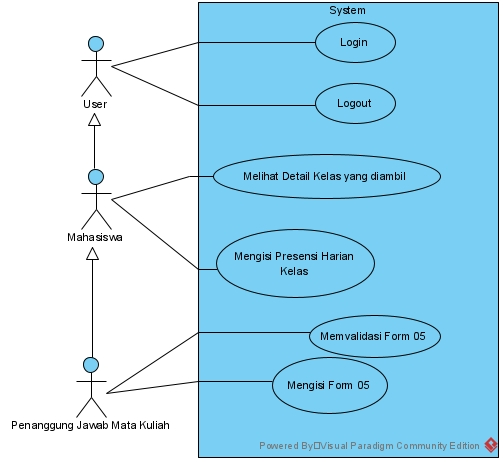
\includegraphics[width=0.8\textwidth]{gambar/diagram/Use Case Iteration 1}
	\caption{Desain \textit{Use Case Diagram Iterasi Pertama}}
	\label{fig:usecase1st}
\end{figure}

Aktor Mahasiswa dapat melihat detail kelas-kelas yang diambil seperti presensi dan nilai setiap mahasiswa pada kelas tersebut dan mengisi presensi pertemuan yang sedang berlangsung.
Aktor Penanggung Jawab Mata Kuliah dapat digeneralisasi menjadi aktor Mahasiswa sehingga mendapat wewenang yang sama seperti aktor Mahasiswa. Aktor penanggung jawab mata kuliah juga dapat mengisi form 05 atau memvalidasi form 05 yang telah dibuat oleh dosen dan memvalidasi presensi form 06 mahasiswa lain.

\textbf{B. \textit{Activity Diagram}}

Dari beberapa \textit{use case} yang telah dibuat, penulis juga membuat \textit{activity diagram} untuk beberapa \textit{use case} yang butuh penjelasan alur untuk menjalankannya. Berikut adalah \textit{activity diagram} yang telah dibuat:

\begin{figure}[h!]
	\centering
	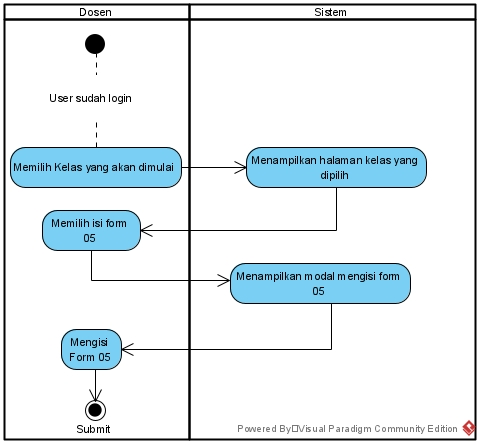
\includegraphics[width=0.7\textwidth]{gambar/diagram/Mengisi Form 05}
	\caption{\textit{Activity} Mengisi Form 05}
	\label{fig:activity2}
\end{figure}

\begin{figure}[h!]
	\centering
	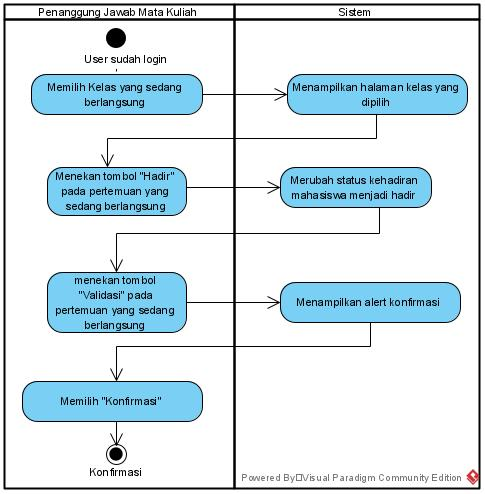
\includegraphics[width=0.7\textwidth]{gambar/diagram/Mengisi Presensi dan Memvalidasi Form 05}
	\caption{\textit{Activity} Mengisi Presensi dan Memvalidasi Form 05}
	\label{fig:activity1}
\end{figure}

Pada gambar \ref{fig:activity2} menggambarkan aktivitas mengisi form 05 yang dapat dilakukan oleh penanggung jawab mata kuliah dan dosen. Pada pengisiannya, penanggung jawab mata kuliah dapat mengosongkan terlebih dahulu materi pembelajaran untuk nantinya ditambahkan oleh dosen.
Pada gambar \ref{fig:activity1} menggambarkan aktivitas mengisi presensi yang dapat dilakukan oleh setiap mahasiswa dan memvalidasi form 05 yang dapat dilakukan oleh penanggung jawab dan dosen.

\textbf{C. Rancangan Tampilan Antarmuka}

Pada rancangan tampilan antar muka program, penulis membuat desain awal dengan menggunakan \textit{tools online}. Pada halaman \textit{login} yang dapat dilihat pada gambar \ref{fig:login}, user mengisi email dan \textit{password} yang terdaftar pada \textit{web service} SIAKAD.

\begin{figure}[h!]
	\centering
	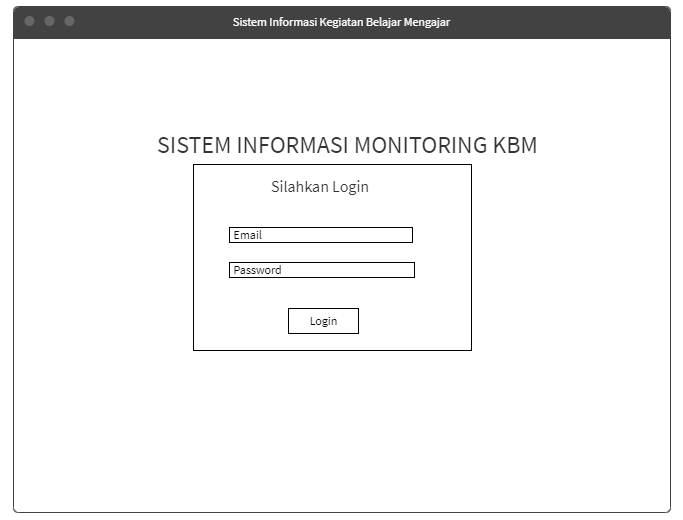
\includegraphics[width=0.8\textwidth]{gambar/mockup/login}
	\caption{Desain Halaman \textit{Login}}
	\label{fig:login}
\end{figure}

Setelah \textit{user} berhasil melakukan \textit{login}, \textit{user} akan dibawa ke halaman \textit{dashboard} dengan menu yang sedikit berbeda bagi setiap jenis \textit{user}. Pada \textit{user} mahasiswa yang dapat dilihat pada gambar \ref{fig:dashboard}, menu yang akan ditampilkan adalah \textit{Home}, Rekap Presensi, dan daftar kelas yang diambil oleh mahasiswa tersebut.

\begin{figure}[h!]
	\centering
	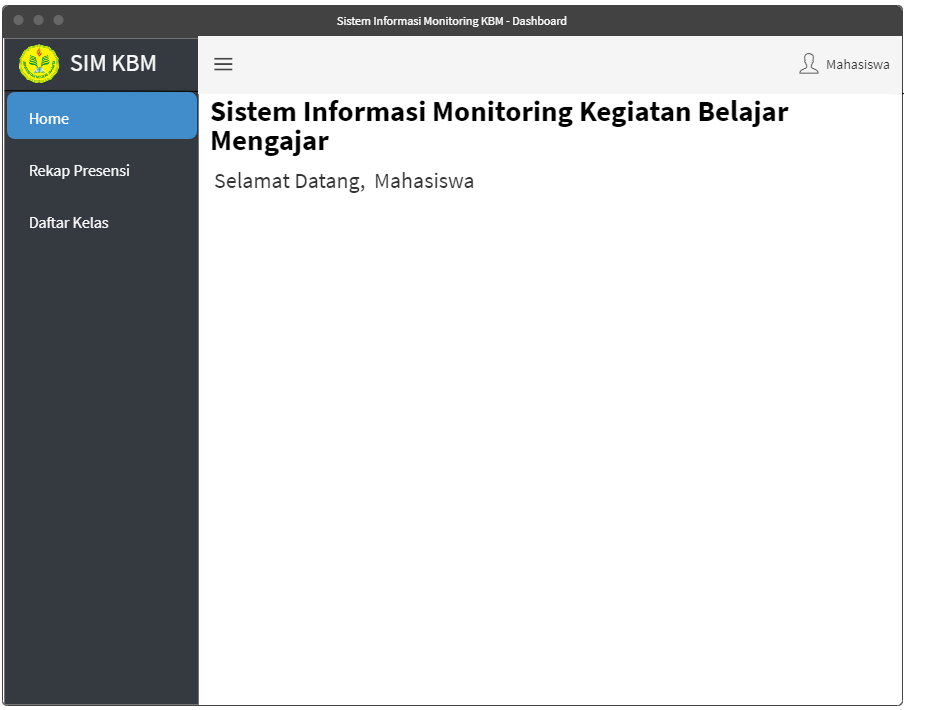
\includegraphics[width=0.8\textwidth]{gambar/mockup/home_mahasiswa}
	\caption{Desain Halaman \textit{Dashboard} Pada mahasiswa}
	\label{fig:dashboard}
\end{figure}

\begin{figure}[h!]
	\centering
	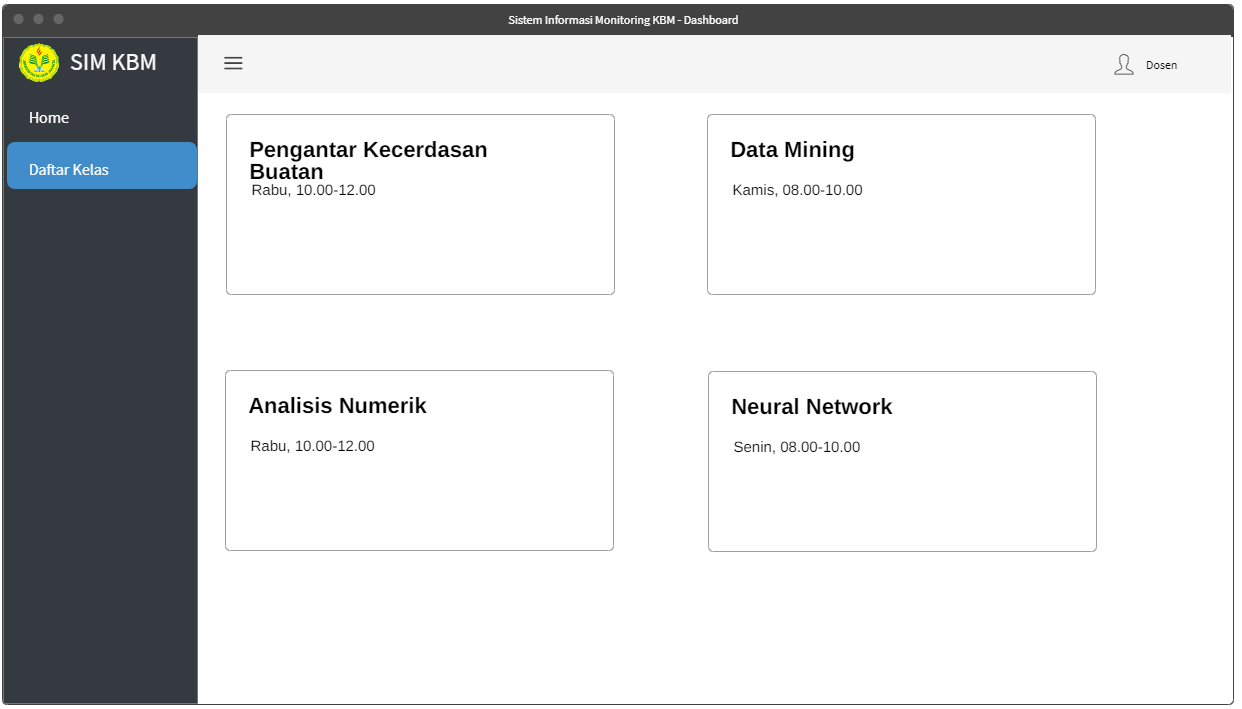
\includegraphics[width=0.8\textwidth]{gambar/mockup/daftar_kelas}
	\caption{Desain Halaman Daftar Kelas}
	\label{fig:daftarkelas}
\end{figure}

Menu Daftar Kelas merupakan menu yang digunakan untuk membuka halaman kelas yang diambil. Halaman Daftar Kelas dapat dilihat pada gambar \ref{fig:daftarkelas}. Menu kelas terdapat empat bagian \textit{tab} di dalamnya, yaitu Pertemuan, Presensi, Tugas, dan Nilai. Pada \textit{tab} pertemuan yang dapat dilihat pada gambar \ref{fig:form05dosen} dosen dapat menambah pertemuan, memvalidasi presensi mahasiswa, dan mengisi pokok bahasan yang dibahas pada pertemuan tersebut. Setelah pertemuan sudah dibuat dan mahasiswa sudah mengisi presensi, dosen juga bisa memvalidasi presensi mahasiswa tersebut. Pada \textit{tab} ini mahasiswa dapat memilih Hadir untuk mengisi presensi pada pertemuan tersebut yang bisa dilihat pada gambar \ref{fig:form05pj}. Penanggung jawab mata kuliah memiliki fungsi tambahan untuk memvalidasi pertemuan yang dibuat oleh dosen.

\begin{figure}[h!]
	\centering
	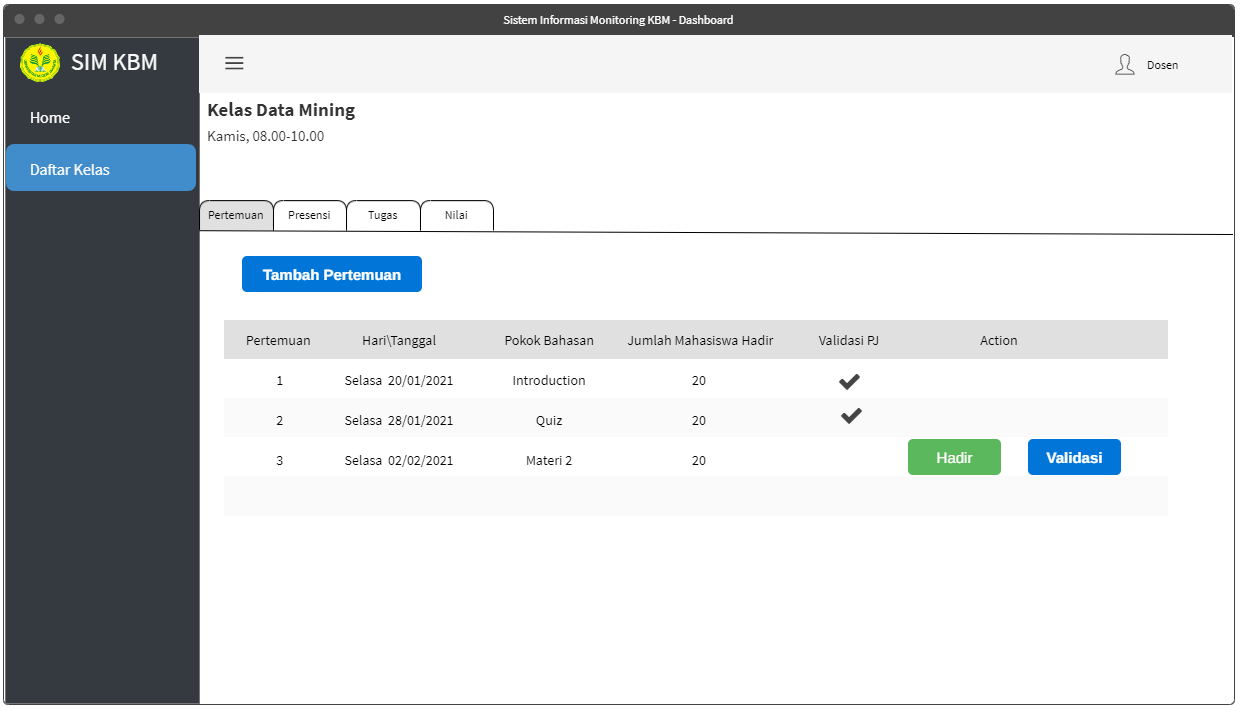
\includegraphics[width=1\textwidth]{gambar/mockup/form05_pj}
	\caption{Desain Halaman Form 05 Pada Penanggung Jawab}
	\label{fig:form05pj}
\end{figure}

\begin{figure}[h!]
	\centering
	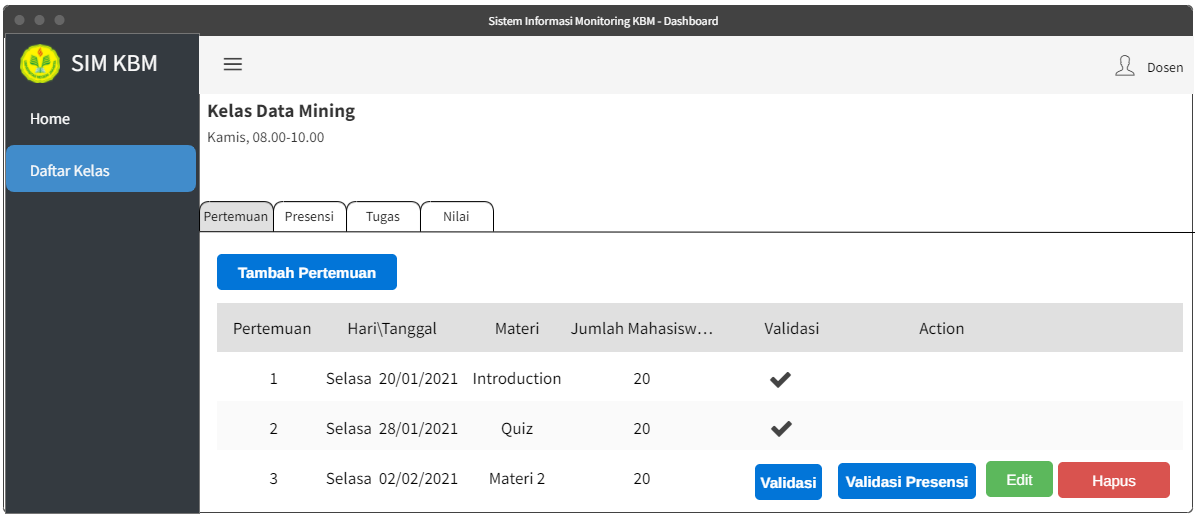
\includegraphics[width=1\textwidth]{gambar/mockup/form05_dosen}
	\caption{Desain Halaman Form 05 Pada Dosen }
	\label{fig:form05dosen}
\end{figure}


\textbf{D. \textit{Class Diagram}}

	Desain \textit{Class Diagram} pada sistem yang dibuat digambarkan dengan mengikuti konsep MVC dimana \textit{class} pada desain dibagi menjadi tiga jenis yaitu \textit{model}, \textit{view}, \textit{controller}. Pada penggunaannya \textit{class} \textit{model} dan \textit{controller} dibuat pada bagian \textit{backend} dengan menggunakan Laravel sedangkan \textit{class view} dibuat pada bagian \textit{frontend} dengan menggunakan \textit{Vue}. Pada diagram berikut ketiga jenis \textit{class} dibedakan dengan menggunakan warna yang berbeda yaitu biru untuk \textit{model}, hijau untuk \textit{view}, dan merah untuk \textit{controller}. Desain \textit{class diagram} pada sistem dapat dilihat pada gambar \ref{fig:classdiagram}

\begin{figure}[H]
	\centering
	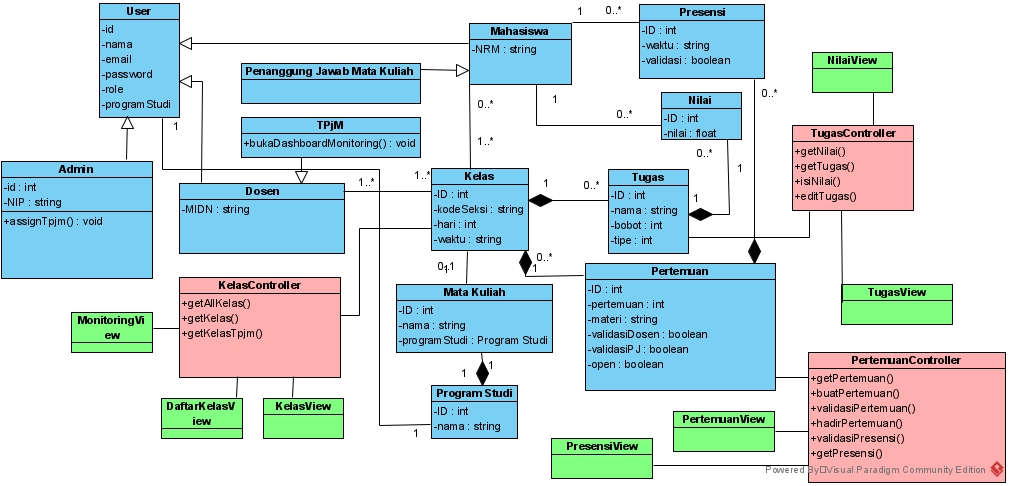
\includegraphics[width=1\textwidth]{gambar/diagram/Class Diagram Fix}
	\caption{Desain Class Diagram}
	\label{fig:classdiagram}
\end{figure}


\textbf{E. \textit{Entity Relationship Diagram}}

	Desain \textit{Entity Relationship Diagram} pada sistem ini dibuat menggambarkan setiap entitas yang digunakan dalam sistem dan relasinya pada \textit{database} dan pada \textit{web service} SIAKAD yang digunakan. Pada ERD tersebut terdapat sebelas entitas dimana enam diantaranya didapatkan dari \textit{web service} dan lima lainnya berada pada \textit{database} sistem ini sendiri. Entitas yang dibuat dan disimpan pada \textit{database} adalah entitas MahasiswaKelas. Absen, Pertemuan, Nilai, dan Tugas. Entitas MahasiswaKelas merupakan \textit{pivot} antara relasi mahasiswa dan kelas yang disimpan karena menyimpan informasi tambahan selain yang didapatkan dari \textit{webservice} yaitu nilai dan \textit{role} penanggung jawab. Entitas Pertemuan dan Absen yang menghubungkan antara mahasiswa dan kelas merupakan entitas yang menggambarkan form 05 dan 06. Desain ERD pada sistem dapat dilihat pada gambar \ref{fig:erd}

\begin{figure}[h!]
	\centering
	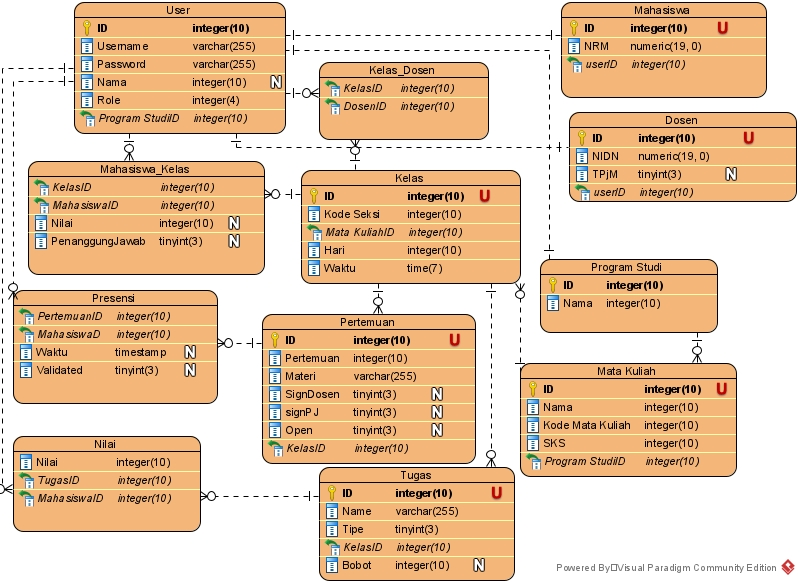
\includegraphics[width=1\textwidth]{gambar/diagram/Entity Relationship Diagram2}
	\caption{Desain Entity Relationship Diagram}
	\label{fig:erd}
\end{figure}

\subsection{Analisis Risiko}
	Pada fase selanjutnya, penulis melakukan analisis risiko yang dapat terjadi pada pengembangan perangkat lunak, dan mencoba mencari solusi yang dapat dilakukan untuk menangani risiko tersebut. Risiko-risiko yang telah teridentifikasi adalah sebagai berikut:
\begin{enumerate}
	\item Penulis tidak memiliki akses \textit{web service} SIAKAD sebagai dosen. 
	\item Relasi basis data yang tidak lengkap karena menggunakan data dari SIAKAD dan tidak menyimpan kembali ke basis data sistem.
	\item Tidak diberikannya dokumentasi dari \textit{web service} SIAKAD
\end{enumerate}
Setelah risiko yang mungkin terjadi teridentifikasi, penulis mendapat beberapa solusi yaitu:
\begin{enumerate}
	\item Meminta dibuatkan akun dosen dan kelas \textit{dummy} untuk melakukan pengembangan pada sisi dosen.
	\item Menggunakan \textit{query} manual untuk mengakses relasi pada basis data.
	\item Membuat list kebutuhan \textit{web service} dan berkomunikasi dengan pihak UPT TIK terkait \textit{web service} yang dibutuhkan.
\end{enumerate}

\subsection{Pengembangan}
	Pada fase pengembangan, penulis melakukan proses pengkodean sekaligus pengujian fitur yang dikembangkan. Hasil dari fase ini adalah perangkat lunak sesuai dengan tujuan yang telah ditentukan. Sebagai fase pertama penulis mulai dengan membuat basis data yang dibutuhkan, lalu membuat \textit{backend} beserta hubungannya dengan \textit{web service} SIAKAD, dan membuat \textit{frontend} atau tampilan. Berikut adalah tampilan-tampilan yang telah dibuat pada fase pengembangan ini.

\begin{figure}[h!]
	\centering
	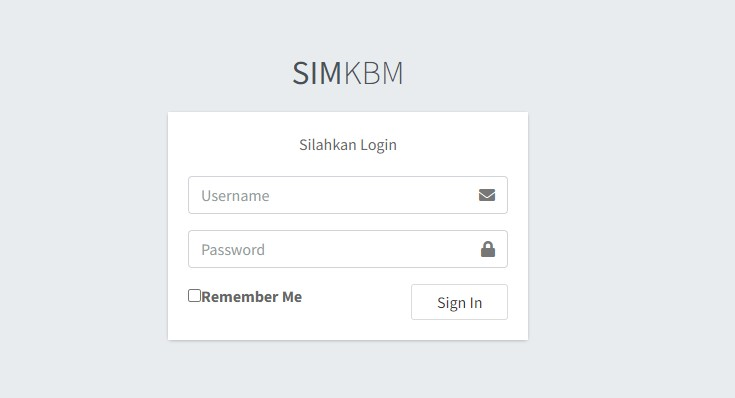
\includegraphics[width=1\textwidth]{gambar/ss/login}
	\caption{Tampilan Halaman \textit{Login}}
	\label{fig:sslogin}
\end{figure}

Gambar \ref{fig:sslogin} adalah tampilan awal ketika membuka \textit{website} Sistem Informasi Monitoring Kegiatan Belajar Mengajar yang merupakan halaman \textit{login}, pengguna dapat mengisi \textit{username} dan \textit{password} akun SIAKAD yang dimiliki. Pengguna juga dapat memilih \textit{Remember Me} untuk masa \textit{login} yang lebih lama. Setelah memilih untuk \textit{Sign In} sistem akan mencoba melakukan \textit{login} ke sistem SIAKAD. Jika \textit{username} dan \textit{password} yang ditulis tidak sesuai dengan akun SIAKAD, akan muncul \textit{alert error}.

\begin{figure}[h!]
	\centering
	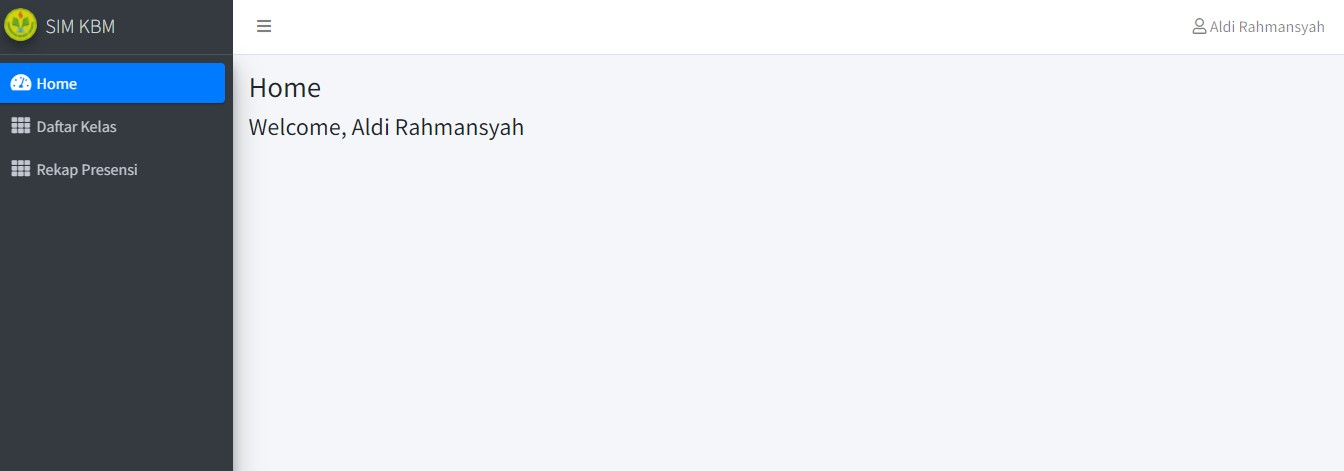
\includegraphics[width=1\textwidth]{gambar/ss/home_mahasiswa}
	\caption{Tampilan Halaman Home}
	\label{fig:sshome}
\end{figure}

\begin{figure}[h!]
	\centering
	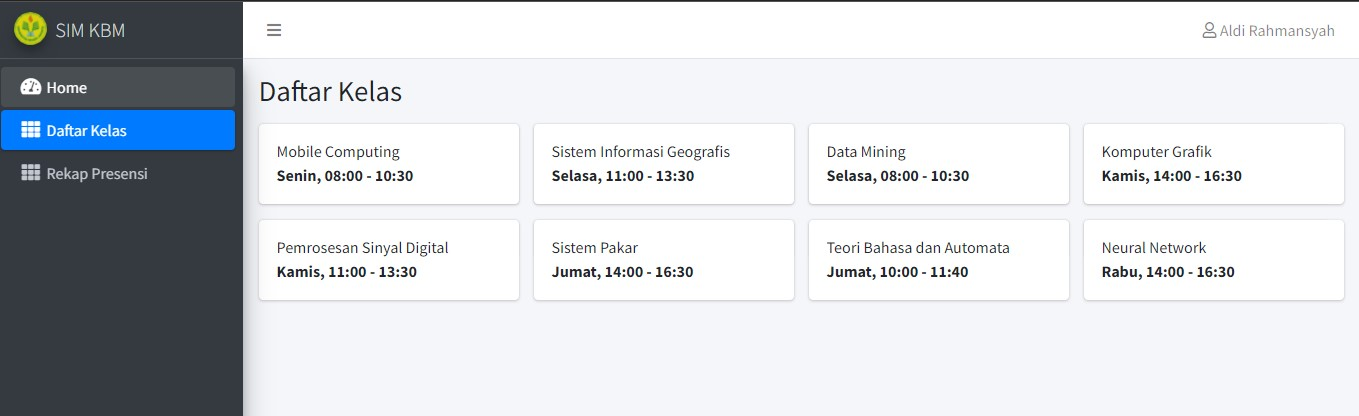
\includegraphics[width=1\textwidth]{gambar/ss/daftar_kelas}
	\caption{Tampilan Halaman Daftar Kelas}
	\label{fig:ssdaftarkelas}
\end{figure}

Gambar \ref{fig:ssdaftarkelas} adalah tampilan Daftar Kelas dimana pengguna dapat melihat daftar kelas yang diampu untuk dosen, atau diambil untuk mahasiswa pada semester yang sedang berlangsung. Pengguna dapat mengeklik salah satu kelas yang ada pada daftar untuk membuka halaman kelas tersebut.

\begin{figure}[h!]
	\centering
	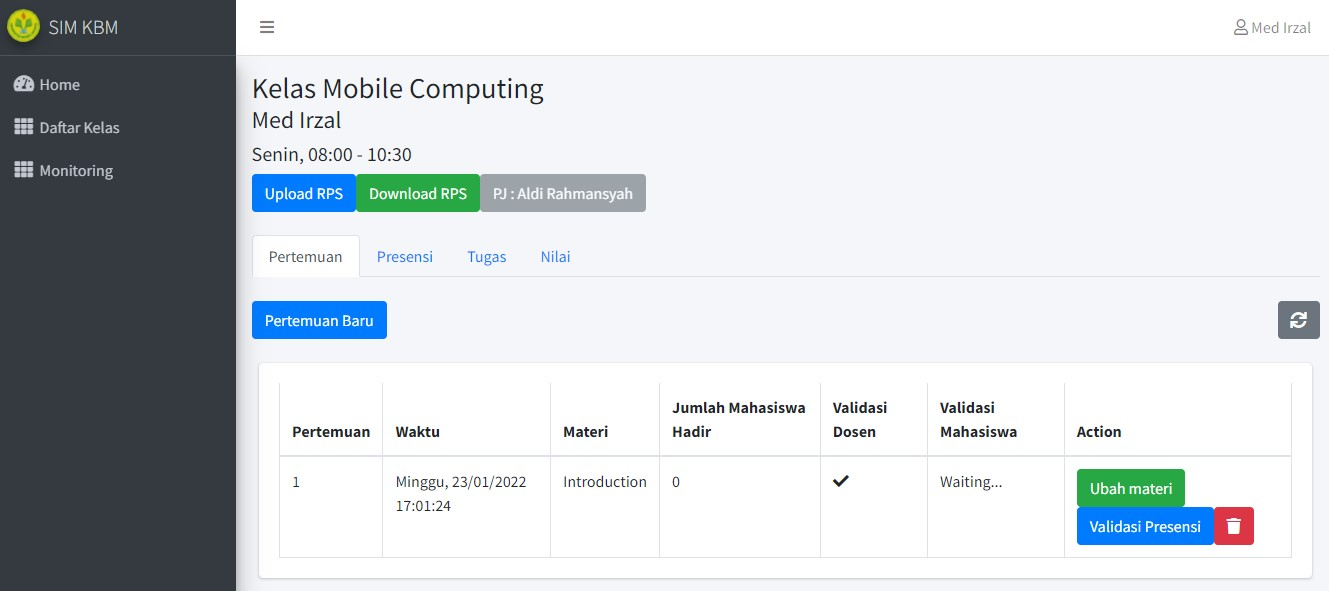
\includegraphics[width=1\textwidth]{gambar/ss/kelas_dosen}
	\caption{Tampilan Halaman Pertemuan Pada Dosen}
	\label{fig:ssform05dosen}
\end{figure}

Gambar \ref{fig:ssform05dosen} adalah tampilan Kelas pada dosen. Pada tampilan ini pengguna dapat mengunduh RPS atau mengunggah RPS dan memilih penanggung jawab kelas jika pengguna adalah dosen pada kelas tersebut. Halaman kelas juga langsung membuka \textit{tab} pertemuan atau form 05. Pada \textit{tab} ini Dosen dapat membuat pertemuan baru, mengubah materi, memvalidasi presensi, atau menghapus pertemuan yang ada. Pada sisi kanan terdapat tombol \textit{reload} untuk memperbarui tabel pertemuan jika ada perubahan.

\subsection{Evaluasi}
	Pada fase evaluasi, penulis melakukan \textit{review} atas iterasi yang telah dilakukan dan merencanakan iterasi yang selanjutnya. Fitur yang dibuat pada spiral ini sudah sesuai dengan rancangan yang dibuat pada fase awal spiral. Untuk iterasi selanjutnya penulis akan mempersingkat waktu iterasi dengan menyelesaikan iterasi tanpa menunggu berakhirnya minggu kedua ketika semua tujuan iterasi sudah tercapai. Pada iterasi selanjutnya penulis akan mengembangkan sisi dosen dan menyempurnakan sisi mahasiswa yang telah dibuat.

%END OF SPS